\chapter{Fundamentação Teórica}
\label{cap:dois}


{\lettrine[loversize=0.25,findent=0.2em,nindent=0em]{A}{liquam} a malesuada magna, et placerat ex. Cras luctus, lorem sit amet semper ornare, nisi libero condimentum elit, ut finibus nunc est et nunc. Proin sollicitudin vulputate placerat. Nam et lacinia arcu, ac cursus neque. Integer facilisis dui nec nibh fringilla sagittis. Morbi blandit enim libero, in consectetur leo consequat ut. Suspendisse a orci id nibh egestas aliquet vel at leo. Etiam at venenatis leo, eget dignissim mi. Donec non justo in erat aliquam molestie eget quis erat. Sed aliquam velit non velit pharetra viverra. Suspendisse dapibus rhoncus ex, at varius ligula condimentum et. Orci varius natoque penatibus et magnis dis parturient montes, nascetur ridiculus mus. Morbi maximus lobortis auctor. Ut et metus lobortis, ultricies dolor et, posuere justo. Mauris a convallis quam. Mauris iaculis gravida ligula, sed viverra quam volutpat nec.

\section{Seção 1}\label{Seção 12}
Donec a nisi lobortis, pretium nulla eu, ornare nulla. Nullam varius iaculis lacus, eu rutrum velit sollicitudin eu. Mauris ultricies lacus vel lectus porta, non laoreet metus maximus. Cras porttitor tincidunt nunc, vel egestas sem. Etiam sit amet ultrices arcu. Sed et lacus quis ex vestibulum fringilla eget a odio. Morbi ut quam pharetra, mattis ipsum a, faucibus neque. Pellentesque laoreet risus eros, eu venenatis ipsum auctor sed. Donec vehicula porttitor nibh, ut sodales est imperdiet pretium. Phasellus quis accumsan odio, id consequat eros. Donec mauris neque, tincidunt vitae sapien finibus, hendrerit tincidunt eros. Integer volutpat sit amet sapien eu mollis. Aliquam erat volutpat. Maecenas porta porttitor mauris et tincidunt. (\citeauthor{smith2014microelectronic}, \citeyear{smith2014microelectronic})

\begin{figure}[h!]
  \caption{Conversor BOOST}
\begin{center}
\resizebox{0.8\textwidth}{!}{
\begin{circuitikz}
 \draw (6.4,-1.2) node[] {$+$};
 \draw (6.4,-1.5) node[] {$v_{o}$};
 \draw (6.4,-1.8) node[] {$-$};
 \draw (0,-3) -- (6,-3);
 \draw (0,-3) [V, l_=$v_{s}$] to (0,0); 
 \ctikzset{diodes/scale=0.6,resistors/scale=0.6}
 \draw (0,0) [L, l^=+ $v_L$ -, -*] to (2,0); 
 \draw (2,-1.8) to[short, *-*] (2,-3);
 \draw (2,0) to[short, -o] (2,-1.3);
 \draw (4,0) -- (6,0);
 \draw (2,0) [D, l^=$D$, *-*] to (4,0); 
 \draw (2,-3) [spst] to (2,0); 
 \draw (4,-3) [C, l_=$C$,*-*] to (4,0); 
 \draw (6,0) [R, l_=$R_L$] to (6,-3); 
 \draw (0.1,-0.1) to[open, f_>=$i_L$] (1.1,-0.1); 
 \draw (2.1,-0.1) to[open, f_>=$i_D$] (3.1,-0.1); 
 \draw (4,0) to[open, f^>=$i_C$] (4,-0.5); 
 \draw (6,0) to[open, f^>=$i_R$] (6,-0.5); 
\end{circuitikz}}\\
  {\footnotesize Fonte: O Autor(2023), adaptado de (\citeauthor{hart2016eletronica}, \citeyear{hart2016eletronica}).}  %Fonte um pouco menor que a do texto
  \label{6.8a.eps}
\end{center}
\end{figure}

Class aptent taciti sociosqu ad litora torquent per conubia nostra, per inceptos himenaeos. Nam porta est sed velit dignissim, ut fringilla est fringilla. Maecenas semper ut dui ac dignissim. Phasellus eu nisl sed diam pellentesque feugiat faucibus nec nisl. Vivamus in tempus dolor. Ut urna diam, lacinia in tincidunt sed, elementum quis velit. Morbi sapien elit, condimentum sed mi eu, ullamcorper tincidunt justo. Aliquam sollicitudin sollicitudin magna ac faucibus.


\section{Seção 2}\label{Seção 22}
Donec a nisi lobortis, pretium nulla eu, ornare nulla. Nullam varius iaculis lacus, eu rutrum velit sollicitudin eu. Mauris ultricies lacus vel lectus porta, non laoreet metus maximus. Cras porttitor tincidunt nunc, vel egestas sem. Etiam sit amet ultrices arcu. Sed et lacus quis ex vestibulum fringilla eget a odio. Morbi ut quam pharetra, mattis ipsum a, faucibus neque. Pellentesque laoreet risus eros, eu venenatis ipsum auctor sed. Donec vehicula porttitor nibh, ut sodales est imperdiet pretium. Phasellus quis accumsan odio, id consequat eros. Donec mauris neque, tincidunt vitae sapien finibus, hendrerit tincidunt eros. Integer volutpat sit amet sapien eu mollis. Aliquam erat volutpat. Maecenas porta porttitor mauris et tincidunt.

Class aptent taciti sociosqu ad litora torquent per conubia nostra, per inceptos himenaeos. Nam porta est sed velit dignissim, ut fringilla est fringilla. Maecenas semper ut dui ac dignissim. Phasellus eu nisl sed diam pellentesque feugiat faucibus nec nisl. Vivamus in tempus dolor. Ut urna diam, lacinia in tincidunt sed, elementum quis velit. Morbi sapien elit, condimentum sed mi eu, ullamcorper tincidunt justo. Aliquam sollicitudin sollicitudin magna ac faucibus.


\section{Seção 3}\label{Seção 32}
Donec a nisi lobortis, pretium nulla eu, ornare nulla. Nullam varius iaculis lacus, eu rutrum velit sollicitudin eu. Mauris ultricies lacus vel lectus porta, non laoreet metus maximus. Cras porttitor tincidunt nunc, vel egestas sem. Etiam sit amet ultrices arcu. Sed et lacus quis ex vestibulum fringilla eget a odio. Morbi ut quam pharetra, mattis ipsum a, faucibus neque. Pellentesque laoreet risus eros, eu venenatis ipsum auctor sed. Donec vehicula porttitor nibh, ut sodales est imperdiet pretium. Phasellus quis accumsan odio, id consequat eros. Donec mauris neque, tincidunt vitae sapien finibus, hendrerit tincidunt eros. Integer volutpat sit amet sapien eu mollis. Aliquam erat volutpat. Maecenas porta porttitor mauris et tincidunt.

\begin{table}
\caption{Coeficientes de $g_4(\alpha)$ para $g_4(\alpha)=\alpha^4+\alpha+1$, em $GF(16)$}
\newcolumntype{?}{!{\vrule width 2pt}}
\centering
\resizebox{0.7\textwidth}{!}{
\begin{tabular}{|c?c|c|c|c|c|c|c|c|c|c|c|c|c|c|c|}
\hline
$n-k$ & $g_{14}$ & $g_{13}$ & $g_{12}$ & $g_{11}$ & $g_{10}$ & $g_9$ & $g_8$ & $g_7$ & $g_6$ & $g_5$ & $g_4$ & $g_3$ & $g_2$ & $g_1$ & $g_0$ \\ \specialrule{2pt}{0pt}{0pt}
  $2$ &     &     &     &     &     &     &     &     &     &     &     &     &  $1$& $6$ & $8$ \\ \hline
  $3$ &     &     &     &     &     &     &     &     &     &     &     &  $1$& $14$& $13$& $12$ \\ \hline
  $4$ &     &     &     &     &     &     &     &     &     &     &  $1$& $13$& $12$& $8$ & $7$ \\ \hline 
  $5$ &     &     &     &     &     &     &     &     &     & $1$ & $11$& $4$ & $6$ & $2$ & $1$  \\ \hline
  $6$ &     &     &     &     &     &     &     &     & $1$ & $7$ & $9$ & $3$ & $12$& $10$& $12$ \\ \hline
  $7$ &     &     &     &     &     &     &     & $1$ & $12$& $13$& $15$& $2$ & $7$ & $14$& $13$ \\ \hline
  $8$ &     &     &     &     &     &     & $1$ & $9$ & $4$ & $3$ & $4$ & $13$& $6$ & $14$& $12$ \\ \hline
  $9$ &     &     &     &     &     & $1$ & $3$ & $1$ & $13$& $9$ & $3$ & $13$& $7$ & $10$& $1$  \\ \hline
 $10$ &     &     &     &     & $1$ & $4$ & $8$ &$10$ & $12$& $9$ & $4$ & $2$ & $12$& $2$ & $7$  \\ \hline
 $11$ &     &     &     & $1$ & $10$ & $5$ & $3$ &$10$ & $13$& $3$ & $15$& $3$ & $6$ & $8$ & $12$ \\ \hline
 $12$ &     &     & $1$ & $5$ & $9$ & $5$ & $8$ & $1$ & $4$ & $13$& $9$ & $4$ & $12$& $13$& $8$  \\ \hline
 $13$ &     & $1$ & $8$ & $5$ & $10$ & $4$ & $3$ & $9$ & $12$& $7$ & $11$& $13$& $14$& $6$ & $2$  \\ \hline
 $14$ & $1$ & $1$ & $1$ & $1$ & $1$ & $1$ & $1$ & $1$ & $1$ & $1$ & $1$ & $1$ & $1$ & $1$ & $1$  \\ \hline

\end{tabular}}\\
{\footnotesize Fonte: O Autor(2023).}
\label{tab:coeficientes de gk(x)}
\end{table}

Class aptent taciti sociosqu ad litora torquent per conubia nostra, per inceptos himenaeos. Nam porta est sed velit dignissim, ut fringilla est fringilla. Maecenas semper ut dui ac dignissim. Phasellus eu nisl sed diam pellentesque feugiat faucibus nec nisl. Vivamus in tempus dolor. Ut urna diam, lacinia in tincidunt sed, elementum quis velit. Morbi sapien elit, condimentum sed mi eu, ullamcorper tincidunt justo. Aliquam sollicitudin sollicitudin magna ac faucibus.


\subsection{Subseção 1}\label{Subseção 12}
Donec a nisi lobortis, pretium nulla eu, ornare nulla. Nullam varius iaculis lacus, eu rutrum velit sollicitudin eu. Mauris ultricies lacus vel lectus porta, non laoreet metus maximus. Cras porttitor tincidunt nunc, vel egestas sem. Etiam sit amet ultrices arcu. Sed et lacus quis ex vestibulum fringilla eget a odio. Morbi ut quam pharetra, mattis ipsum a, faucibus neque. Pellentesque laoreet risus eros, eu venenatis ipsum auctor sed. Donec vehicula porttitor nibh, ut sodales est imperdiet pretium. Phasellus quis accumsan odio, id consequat eros. Donec mauris neque, tincidunt vitae sapien finibus, hendrerit tincidunt eros. Integer volutpat sit amet sapien eu mollis. Aliquam erat volutpat. Maecenas porta porttitor mauris et tincidunt.

\begin{figure}[h!]
\caption{Formas de onda.}
\begin{center}
  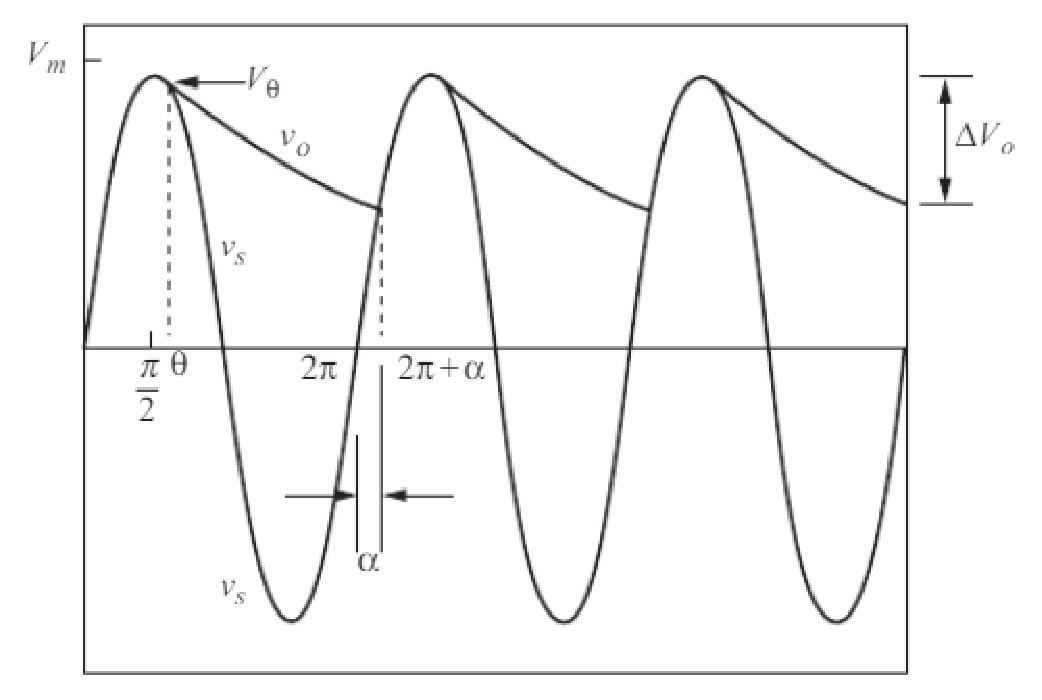
\includegraphics[width=7cm]{Ilustrações/Forma_de_onda.eps}\\
  {\footnotesize Fonte: (\citeauthor{hart2016eletronica}, \citeyear{hart2016eletronica}).}
  \label{3.2b.eps}
\end{center}
\end{figure}

Class aptent taciti sociosqu ad litora torquent per conubia nostra, per inceptos himenaeos. Nam porta est sed velit dignissim, ut fringilla est fringilla. Maecenas semper ut dui ac dignissim. Phasellus eu nisl sed diam pellentesque feugiat faucibus nec nisl. Vivamus in tempus dolor. Ut urna diam, lacinia in tincidunt sed, elementum quis velit. Morbi sapien elit, condimentum sed mi eu, ullamcorper tincidunt justo. Aliquam sollicitudin sollicitudin magna ac faucibus.




